
\section{Where do big time differences arise between slalom skiers? }
The goal for alpine skiers is to ski a slalom course marked by gates in the shortest possible time. These slalom courses never consist of a single situation repeated from turn to turn. Instead, they include various sections with different terrains and incline angles, gate placements, snow conditions, winds, and visibility. Consequently, no two turns are the same, and the skiers must master a vast array of situations to perform well. 

At first glance, the differences between the top skiers and the next-best skiers might seem marginal. For instance, it is not uncommon for the gap between the best performer and the next ten competitors to be less than a second on a 50-second slalom course. A natural assumption is that these small differences are consistent throughout the course. However, a closer examination of specific sections of the course—through gate-to-gate analysis or shorter intermediate section analysis—reveals significant disparities in certain segments\cite{supej_relations_2006, reid_kinematic_2010, supej_new_2011, supej_mechanical_2011, federolf_quantifying_2012}. These differences suggest that athletes have both strong and weak areas that can be targeted and improved through training.

Previous slalom studies have identified three crucial sections: the start, the hairpins, and the flat sections\cite{supej_new_2011}. Among these, the flat section typically makes up the largest proportion of the total course (see Fig. \ref{fig: flatcourse} for an illustration). Consequently, improvements in this section could have a more substantial impact on a skier's overall performance compared to the start or hairpin turns. Furthermore, strategies effective on flat terrain may be applicable to hairpin turns. Therefore, for my doctoral project, I chose to focus on the flat section as the area for further study.

\begin{figure}
    \centering
    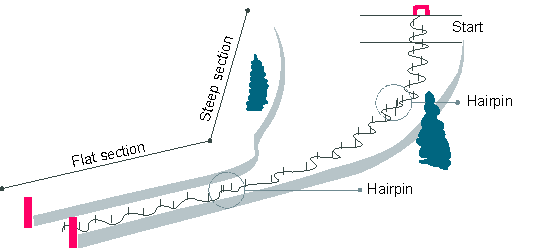
\includegraphics[width=1\linewidth]{figure/figure_introduction_course.pdf}
    \caption{Illustration of different section in a slalom race}
    \label{fig: flatcourse}
\end{figure}

\section{What can skiers do to improve their performance in flat sections in slalom?}
The next question is how skiers can increase their speed on flat sections in slalom. In this sport, performance boils down to how effectively athletes can utilize the mechanical energy available to them \cite{supej_differential_2008, supej_how_2010}. Therefore, this section first outlines the fundamental mechanical energy principles of skiing. Based on these principles and quantitative evidence from field research on elite skiers, I will propose four strategies to potentially enhance skier performance on flat terrain in slalom, which we wanted to study in this doctoal project.  

\subsection{Energy mechanics of alpine skiing}\label{introduction: energymechanics}
When skiers take the ski lift to the top, they  accumulate gravitational potential energy. This acquired potential energy is the skier's main engine \cite{supej_differential_2008, supej_mechanical_2011} and enables them to do work such as making the ski penetrate the snow to make it turn. The amount of potential energy available to the skier for performing such work at the top of a slalom course can be derived from the following equation:
\[U=mgh\]
Here, $U$ represents the gravitational potential energy (measured in joules), $m$ represents the mass of the skier (measured in kilograms), g represents the gravitational acceleration (approximately $m/s^2$) acting on the skier, and $h$ represents the height (measured in meters). When the skier descends the slalom course, the amount of work done by gravity can be derived by finding the gravitational potential energy for the initial position $U_1$ (e.g., at the top of the slalom course) and the gravitational potential energy for the final position $U_2$ (e.g., at the end of the first turn); then, the negative change in potential energy can be calculated: 
\[W=-U_2 + U_1\]
\[W= -\Delta U \]
This quantity represents the work of gravity on the skiers as they descend from the top to the lower position of the slalom course. According to the law of conservation of mechanical energy, all this work must be converted to kinetic energy when gravity is the sole force acting on the skier. The skiers' kinetic energy can be represented by the following equation:
\[ K = \frac{1}{2} m v^2 \]
where $K$ is the kinetic energy, $m$ is the mass of the skier, and $v$ is the velocity of the skier. Consequently, the sum of the potential and kinetic energy  (denoted as $E$ for mechanical energy) remains constant during a descent, as expressed by the following equation:
\[ E = U + K \]
During descents, however, skiers are exposed to two dissipative forces that oppose motion and can result in some loss of energy transfer to kinetic energy. For skiers, these two dissipative forces are air drag and snow friction (collectively denoted as $D$)\cite{supej_differential_2008}. Therefore, the total mechanical energy during a descent equals the sum of the kinetic energy and the dissipating forces (equation below), and is conceptually illustrated in Fig. \ref{fig:energy}.
\[ U = K + D\]
Consequently, in terms of the mechanical energy principle, a skier's goal during a descent should be to maintain high kinetic energy \cite{supej_differential_2008, supej_mechanical_2011, supej_how_2010}. One conventional strategy that most skilled skiers' employ to achieve this goal include carving instead of skidding \cite{supej_differential_2008, supej_relations_2006, reid_kinematic_2010, reid_turn_2009}. Are there solutions that can effectively improve performance on this section beyond the usual strategy? 

\begin{figure}[H]
    \centering
    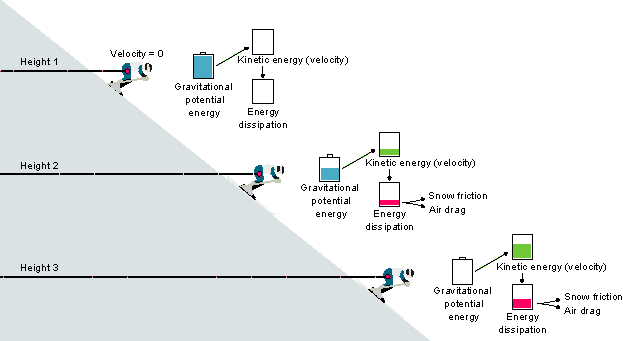
\includegraphics[width=1\linewidth]{figure/figure_introduction_mechenergy3.pdf}
    \caption{Illustration of mechanical energy in alpine skiing}
    \label{fig: energy}
\end{figure}



\subsection{Strategies to improve race times in flats in slalom}\label{introduction: strategies}
If most skilled skiers can execute clean, carved turns, what else can they do to achieve better performance on flats in slalom? Here, I outline four strategies that can potentially achieve this goal, all directed at improving energy mechanics management.  Fig. \ref{fig: strategies} illustrates these four strategies.  

The first strategy skiers could potentially use to maintain high kinetic energy during a turn and therefore improve their race times on flat sections in slalom is the 'stand against' technique. This strategien er nokså utbredt blant trenere i skimiljøet, og går ut på at skiers maintain a stable stance and actively resist being compressed toward their bindings by centrifugal force during a turn (from the skier's frame of reference). According to Lind and Sander's theoretical model on 'pumping to increase velocity' \cite{lind_physics_2013}, this active force resistance could minimize skiers' kinetic energy loss during a slalom turn by keeping the moment of inertia about the axis of rotation fixed instead of increasing it, as would occur if the skier collapsed during the turn. In their model, the rotational kinetic energy of a ski turn can be represented by the following equation: 
\[ T = \frac{L^2}{2I} \]
Here, $T$ represents the kinetic energy of rotation, and $L$ represents the angular momentum (that is, angular velocity ($\omega$) multiplied by the moment of inertia about the axis of rotation ($I = mr^2$)). Lind and Sanders considered a rider traveling on a cart on a friction-free rail with a curved turn and no torque to act on the system. In this situation, if the rider were to collapse toward the cart due to the centrifugal force, the moment of inertia would increase by lengthening the radius about the axis of rotation. Consequently, some rotational kinetic energy is lost if the skier fails to resist the centripetal force. Stand against might therefore be an effective strategy to ski faster on flats in slalom.  

A second and perhaps better strategy skiers can employ to maintain high kinetic energy during a turn is to 'rock skis forward'. By shifting their vertical position forward and backward, skiers regulate the ski’s total pressure distribution exerted against the snow\cite{lemaster_skiers_1999, lemaster_ultimate_2010, howe_new_2001}. This regulation not only helps skiers maintain balance but also affects the ski's turning behavior. For example, when skiers edge their skis, moving the center of mass toward the tip of the ski increases the pressure distribution on the ski's forebody, enabling it to turn more sharply. Conversely, if skiers edge their skis but shift their center of mass backward to the ski's tail, they decrease the pressure at the ski's forebody and consequently make the turn more gradual \cite{lemaster_skiers_1999, lemaster_ultimate_2010}. In ski racing, skiers generally aim to turn more sharply in the beginning and during the turn and should therefore shift their center of mass to distribute the pressure to the ski's forebody to make it engage with the snow. However, after gate passage, skiers generally aim to stop turning and should therefore shift their center of mass backward by rocking the skis forward. By rocking the skis forward after gate passage, skiers could in principle counteract the unnecessary loss of kinetic energy caused by the skis penetrating and digging unnecessarily into the snow in the exit of the turn. In support of this, previous research has found a strong linear relationship between the skier's forward position and energy dissipation \cite{reid_turn_2009, reid_kinematic_2010}. Additionally, faster skiers have shown to rock their skis more forward and pressure the back part of the ski for considerably longer during a turn compared to slower skiers\cite{reid_kinematic_2010, tjorhom_beskrivelse_2007}. Consequently, rocking skis forward could be an even better strategy than the stand against strategy for improving race times on flat terrain in slalom. 

The third strategy that can potentially make skiers faster on flat slopes in slalom is to 'extend,' also referred to as 'pumping' to increase velocity \cite{lind_physics_2013}. This strategy involves skiers moving their center of mass closer to the axis of rotation of a turn from a laterally inclined position by extending their legs. When the skiers extend this way, they can increase their kinetic rotational energy under certain situations. According to Lind and Sanders \cite{lind_physics_2004} model, the skier achieves this effect by shortening the radius of the axis about which they rotate, which will reduce the moment of inertia and consequently increase the rotational kinetic energy of the system under the assumption that angular momentum is conserved. In their model, the gain in rotational kinetic energy from this motion is proportional to the amount of work the skier does against the centrifugal force (from the skier's frame of reference); therefore, a larger extension movement will accomplish a greater increase in rotational kinetic energy. Scientists have previously assumed that the contribution of pumping to increase the velocity through a turn is minimal and an negotiable mechanism to leverage to improve skiers' race times\cite{supej_differential_2008}. Critics are directed that Lind and Sander's model neglects friction and that it only should work with low speeds \cite{supej_differential_2008, supej_how_2010}. Nevertheless, several studies has been observed that skilled alpine skiers gain additional kinetic energy at the exit of the turn—an increase that cannot be accounted for solely by their available potential energy at that moment\cite{reid_kinematic_2010, supej_how_2010, supej_differential_2008}. Moreover, in an experiment we conducted in 2012, elite skiers had better race times on a flat slalom section when they skied the course with the pumping technique than when they skied the section straight down, despite taking a significant longer trajectory in skiing the course. Therefore, "extend" could be a very important strategy.  

The final strategy is to "extend with rock skis forward", which combines "extend" and "rock skis forward". In a simulation study of skiers pumping on a an undulating terrain, this was the the best performing strategy \cite{mote_accelerations_1983}, and it has been suggested that this could be the best strategy to perform in slalom turns in certain situations \cite{reid_kinematic_2010}. We therefore considered this strategy as the theoretical best strategy. 

Although mechanical theory and quantitative evidence suggest that 'extend with rock skis forward' is an effective strategy on flat terrain in slalom, no or little experimental data on this topic exist. Et viktig spørsmål med doktorgraden var derfor å finne ut hvilke strategier gode skikjørere presterer best med på flater. D


Another important goal was to understand the impact of a training intervention focused on the pumping (or extend) strategy exerted on the kinematics of skiers. If skiers can pump themselves to higher velocities, it is crucial to investigate the kinematic changes involved. This understanding will help us better grasp what actually occurs when skiers pump. Therefore, another question was: what happens to a skier's kinematics when they learn to pump?


\begin{figure}[H]
    \centering
    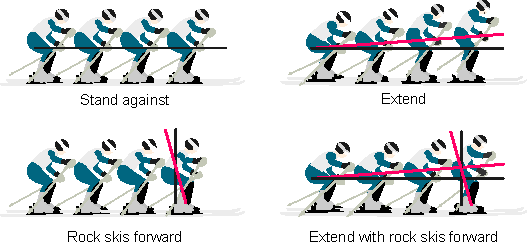
\includegraphics[width=1\linewidth]{figure/figure_introduction_strategies.pdf}
    \caption{Illustration of the strategies to improve reace times in flats in slalom}
    \label{fig: strategies}
\end{figure}



\section{What is the best way to teach these skills?}
The next question is whether insights from cognitive science can help coaches create more effective training. To ensure effective training, coaches generally have two main strategies for creating optimal learning situations at their disposal: designing learning problems for athletes and using effective teaching signals for instruction and feedback. In alpine skiing, skiers constantly face new slalom courses in races, requiring them to adapt their strategies and techniques. Therefore, their training should cover a wide variety of course scenarios to best prepare them to handle these diverse demands effectively. Given that coaches address this breadth of variation, should they also increase the frequency at which they expose their skiers to new learning problems? This is one of the questions we aim to test in this doctoral study. Another question is whether coaches can improve their use of instruction and feedback by selecting the most effective teaching signals.


\subsection{Can coaches improve skill learning by increasing the frequency at which they expose skiers to new learning problems?}
One learning effect that supports increasing the frequency at which coaches or teachers expose skiers to new learning problems is the contextual interference effect \cite{lee_contextual_2012, shea_contextual_1979, magill_review_1990}. This teaching strategy involves training learning problems (in our case courses) in a nonrepetitive sequence (that is, interleaved order), such as practicing learning problems A, B, and C in the order of BCA, ACB, or ABC, rather than a practice structure where problems are repeated in blocks (that is, blocked practice), such as AAA, BBB, or CCC. This nonsystematic training structure has been shown to be an effective teaching strategy for improving skill retention and transfer in various simple learning tasks \cite{tsutsui_contextual_1998, simon_metacognition_2001, shea_context_1983, shea_contextual_1979, tsay_signatures_2023}.

Two main explanations have been proposed to account for the contextual interference effect: the elaboration hypothesis \cite{shea_contextual_1979, shea_context_1983} and the reconstruction/forgetting hypothesis \cite{lee_can_1985, lee_locus_1983}. The elaboration hypothesis proposes that interleaved practices prompt individuals to process information more eloborately during acquisition, which enriches their understanding and problem solving techniques. This increased elaboration process enhances retention, which is not fully realized when practicing learning problems in a blocked order \cite{shea_contextual_1979, shea_context_1983}. In contrast, the reconstruction/forgetting hypothesis posits that increased problem switching provides more opportunities to forget task-relevant information held in working memory. This forgetting of task-relevant information forces the learner to reconstruct the action plan for every trial the learner revists the task. The repetitive process of abandoning and reconstructing action plans during interleaved practice contributes to better memory formation and thus increased retention \cite{lee_can_1985, lee_locus_1983}.

The contextual interference effect has not always succeeded in transferring to the learning of real-world skills, however \cite{wulf_principles_2002, brady_theoretical_1998, barreiros_contextual_2007, AMMAR2023100537, guadagnoli_challenge_2004}. This discrepancy can be understood through the challenge-point framework \cite{guadagnoli_challenge_2004} and recent extensions of it \cite{hodges_extended_2022}, where the effect of contextual interference is moderated by both the difficulty of the task and the skill level of the performer. In this framework, easy tasks can benefit from contextual interference to make the task more challenging, whereas difficult tasks are already challenging enough to serve as adequate learning stimuli on their own and are best learned without contextual interference initially. As the learner becomes more skilled, the learning process may benefit from increased contextual interference to improve the level of difficulty. In align with this prediction, studies have shown that beginners who learn skills when practice increases from blocked to interleaved practice learn better than those who use blocked or interleaved practice alone \cite{porter_systematically_2010, saemi_practicing_2012}. 

One prediction derived from the challenge point framework is that skilled athletes can benefit from interleaved practice to make training more challenging and therefore better. Consistent with this notion, \cite{hall_contextual_1994} found that skilled baseball players who practiced batting achieved better retention through interleaved practice than through blocked practice. In contrast, \cite{buszard_quantifying_2017} found no statistically significant differences in retention between tennis players learning to serve through interleaved practice and those using blocked practice. Instead, these researchers found evidence for improved transfer to new situations. Thus, it is not entirely clear whether contextual interference can be generalized to skilled performers. One idea is that contextual interference is more beneficial in open sports, where performers must constantly switch between different strategies to solve tasks, potentially making it important for alpine skiers \cite{farrow_chapter_2017, buszard_quantifying_2017}. An important aim of this study is to investigate whether the contextual interference effect can be used to improve the training of skilled performers. 

\subsection{Can coaches improve their instruction and feedback using reinforcement learning?}
Den andre treningsstrategien trenere kan bruke for å skape gode læringsbetingelser er gjennom gjennom teaching signalet de bruker for instruksjon og tilbakemeldinger. Although we exercise caution in generalizing and asserting that all coaches teach in a specific way, er det vanlig formen for teaching signal trenere bruker er instruksjonsbasert teaching \cite{williams_practice_2005, williams_effective_2023, hodges_modelling_2002}. In this approach, they offer performers a correct solution followed by corrective feedback. For instance, a ski coach may encourage the skier to take a shorter line around the gate and then further encourage the learner to shorten the line after a few trials. This teaching strategy can be likened to supervised learning in motor learning, where the difference between the desired strategy and the performer's movement outcome represents a teaching signal for skill improvement  \cite{jordan_forward_1992, wolpert_motor_2010, doya_complementary_2000}. Through practice, this teaching signal can bring the performer closer to executing what is assumed to be the correct choice. But is this teaching strategy truly the most effective approach for enabling learners to select and employ effective strategies? 

Supervised learning offers a promising approach for assisting learners in making informed strategy choices, yet it may also lead learners away from discovering the optimal strategy. First, the coach's advice may not be the optimal solution, as the strategy that coaches believes to be optimal does not always align with reality, even for the best-trained eye \cite{supej_impact_2019, cochrum_visual_2021}. Consequently, learners might be hindered to learn the best strategy when coaches opt for suboptimal strategies \cite{gray_plateaus_2017}. Worse, these learned suboptimal strategies might turn into habits that can be difficult to break \cite{popp_effect_2020}. Second, learners trained through supervised learning might also be constrained to adopting a single ('universal') strategy for all situations rather than acquiring a repertoire of strategies and discerning the most effective strategies for each specific scenario. Finally, it remains uncertain whether the prescriptive approach is the most effective teaching strategy for enabling performers to achieve long-lasting learning effects \cite{wulf_instructions_1997, hodges_role_1999, williams_practice_2005,williams_effective_2023}. 

Another, yet much less frequently adopted, teaching strategy to help learners learn to make good choices is through reinforcement learning \cite{sutton_reinforcement_2018}. The cornerstone of this approach is that the learner learns from evaluations instead of instruction, which occurs by using successes and failures of outcomes as teaching signals. That is, the performer learns the value of different strategies which allows them to finally pick the best solution, rather than being told the putatively correct solution to the problem. Specifically, these values are learned by comparing a given choice's outcomes with the choice's currently expected outcome. Outcomes that exceed or fall short of expectations result in errors in reward prediction, signaling that the learner must update their predictions to better anticipate future rewards following that action \cite{rescorla_theory_1972}. These reward prediction errors are then incorporated to form a new and better estimate of expected reward by updating expectations through a weighted running average. The computations underlying this form of value-learning of choices have been tremendously powerful in explaining human and animal learning \cite{waelti_dopamine_2001, schultz_neural_1997, pessiglione_dopamine-dependent_2006,lee_neural_2012, law_reinforcement_2009, tobler_human_2006} as well as training AI to perform complex tasks such as computer games starting from pixel inputs, only\cite{mnih_human-level_2015}. In addition, reinforcement learning has been shown to improve motor skill learning on simple tasks performed in the laboratory \cite{lior_shmuelof_overcoming_2012, abe_reward_2011, truong_error-based_2023, hasson_reinforcement_2015}. Based on this evidence, we ask whether reinforcement learning offers a better alternative for training learners to make better decisions about strategies than traditional supervised learning with a coach. 

